\def\year{2020}\relax
%File: formatting-instruction.tex
\documentclass[letterpaper]{article} % DO NOT CHANGE THIS
\usepackage{aaai20}  % DO NOT CHANGE THIS
\usepackage{times}  % DO NOT CHANGE THIS
\usepackage{helvet} % DO NOT CHANGE THIS
\usepackage{courier}  % DO NOT CHANGE THIS
\usepackage[hyphens]{url}  % DO NOT CHANGE THIS
\usepackage{graphicx} % DO NOT CHANGE THIS
\urlstyle{rm} % DO NOT CHANGE THIS
\def\UrlFont{\rm}  % DO NOT CHANGE THIS
\usepackage{graphicx}  % DO NOT CHANGE THIS
\frenchspacing  % DO NOT CHANGE THIS
\setlength{\pdfpagewidth}{8.5in}  % DO NOT CHANGE THIS
\setlength{\pdfpageheight}{11in}  % DO NOT CHANGE THIS

%%%%%%%%%%%%%%%%%%%%%%%%%%%%%%%%%
% Ryan's packagages
\usepackage{algorithmicx} % Used for writing algorithms
\usepackage{algpseudocode} % Default algorithm psedocode for algorimicx



%\nocopyright
%PDF Info Is REQUIRED.
% For /Author, add all authors within the parentheses, separated by commas. No accents or commands.
% For /Title, add Title in Mixed Case. No accents or commands. Retain the parentheses.
 \pdfinfo{
/Title (ARO:  A Memory-Based Approach to Environments with State Aliasing)
/Author (Ryan Regier, Owen Price, Alex Hadi, Zachary Faltersack and Andrew Nuxoll)
}

%Leave this	
% /Title ()
% Put your actual complete title (no codes, scripts, shortcuts, or LaTeX commands) within the parentheses in mixed case
% Leave the space between \Title and the beginning parenthesis alone
% /Author ()
% Put your actual complete list of authors (no codes, scripts, shortcuts, or LaTeX commands) within the parentheses in mixed case. 
% Each author should be only by a comma. If the name contains accents, remove them. If there are any LaTeX commands, 
% remove them. 

% DISALLOWED PACKAGES
% \usepackage{authblk} -- This package is specifically forbidden
% \usepackage{balance} -- This package is specifically forbidden
% \usepackage{caption} -- This package is specifically forbidden
% \usepackage{color (if used in text)
% \usepackage{CJK} -- This package is specifically forbidden
% \usepackage{float} -- This package is specifically forbidden
% \usepackage{flushend} -- This package is specifically forbidden
% \usepackage{fontenc} -- This package is specifically forbidden
% \usepackage{fullpage} -- This package is specifically forbidden
% \usepackage{geometry} -- This package is specifically forbidden
% \usepackage{grffile} -- This package is specifically forbidden
% \usepackage{hyperref} -- This package is specifically forbidden
% \usepackage{navigator} -- This package is specifically forbidden
% (or any other package that embeds links such as navigator or hyperref)
% \indentfirst} -- This package is specifically forbidden
% \layout} -- This package is specifically forbidden
% \multicol} -- This package is specifically forbidden
% \nameref} -- This package is specifically forbidden
% \natbib} -- This package is specifically forbidden -- use the following workaround:
% \usepackage{savetrees} -- This package is specifically forbidden
% \usepackage{setspace} -- This package is specifically forbidden
% \usepackage{stfloats} -- This package is specifically forbidden
% \usepackage{tabu} -- This package is specifically forbidden
% \usepackage{titlesec} -- This package is specifically forbidden
% \usepackage{tocbibind} -- This package is specifically forbidden
% \usepackage{ulem} -- This package is specifically forbidden
% \usepackage{wrapfig} -- This package is specifically forbidden
% DISALLOWED COMMANDS
% \nocopyright -- Your paper will not be published if you use this command
% \addtolength -- This command may not be used
% \balance -- This command may not be used
% \baselinestretch -- Your paper will not be published if you use this command
% \clearpage -- No page breaks of any kind may be used for the final version of your paper
% \columnsep -- This command may not be used
% \newpage -- No page breaks of any kind may be used for the final version of your paper
% \pagebreak -- No page breaks of any kind may be used for the final version of your paperr
% \pagestyle -- This command may not be used
% \tiny -- This is not an acceptable font size.
% \vspace{- -- No negative value may be used in proximity of a caption, figure, table, section, subsection, subsubsection, or reference
% \vskip{- -- No negative value may be used to alter spacing above or below a caption, figure, table, section, subsection, subsubsection, or reference

\setcounter{secnumdepth}{0} %May be changed to 1 or 2 if section numbers are desired.

% The file aaai20.sty is the style file for AAAI Press 
% proceedings, working notes, and technical reports.
%
\setlength\titlebox{2.5in} % If your paper contains an overfull \vbox too high warning at the beginning of the document, use this
% command to correct it. You may not alter the value below 2.5 in
\title{ARO:  A Memory-Based Approach to Environments with State Aliasing }
%Your title must be in mixed case, not sentence case. 
% That means all verbs (including short verbs like be, is, using,and go), 
% nouns, adverbs, adjectives should be capitalized, including both words in hyphenated terms, while
% articles, conjunctions, and prepositions are lower case unless they
% directly follow a colon or long dash


%%\author{Author's Names Omitted for Peer Review
\author{Ryan Regier, Owen Price, Alex Hadi, Zachary Faltersack and Andrew Nuxoll \\ 
University of Portland\\ %If you have multiple authors and multiple affiliations
5000 North Willamette Boulevard\\
Portland, Oregon 97203\\
engineering@up.edu % email address must be in roman text type, not monospace or sans serif
}


\begin{document}

\maketitle

\begin{abstract}

In order to integrate machine learning and knowledge engineering, it
is necessary to store both learned and engineered knowledge in a
common format that can be used by an agent to make intelligent
decisions. Such integration is much more useful in data sparse
environments, where traditional machine learning techniques fail.  In
this paper, we will define a rule structure that stores patterns of
cause and effect. These rules can easily embed expert knowledge on
causal relationships. We will then present ARO, an algorithm for
learning rules and using rules to navigate data sparse
environments. Our results show that ARO is more effective than other
known solutions to this problem. ARO has the additional advantages
that it more easily integrates with knowledge engineering techniques
and uses no hyperparameters.

\end{abstract}

\noindent




\section{Background}

In environments with an abundance of data, machine learning agents are
effective at learning patterns, even those not known by experts in the
domain. However, in data-sparse environments, traditional machine
learning agents fail \cite{Chrisman92}. We find that this kind of
environment would be ideal for the integration of knowledge
engineering with machine learning techniques. One such environment is
the Blind Finite State Machine environment.  In this environment, the
agent navigates a finite state machine (FSM) \cite{Hopcroft06} to
reach a goal state.  The machine is designed so that the agent can
reach the goal from any state (no dead ends) but otherwise the
transition table is randomly generated.  Upon reaching the goal the
agent is immediately moved to a randomly selected, non-goal state and
informed of its success.  Thus the agent knows when it reaches the
goal but can never actually take an action in the goal state.

The task seems trivial at first.  However, it is greatly complicated
because the agent is only aware of the following:
\begin{itemize}
\item the FSM alphabet (available actions)
\item a goal sensor indicating when it reaches the goal
\end{itemize}

\bigskip  %vertical space here makes this more readable

Specifically, the agent is \underline{not} aware of the following:
\begin{itemize}
\item the number of states
\item what state it currently is in
\item the transition table of the FSM
\end{itemize}

The agent repeatedly performs the task in a given FSM and its success
is measured by how many states it takes to reach the goal at each
iteration.  Experiments with human subjects (not published) indicate
that this task is exceptionally difficult for humans.

In such an environment, a traditional machine learning agent is unable
to learn effective behavior.  Such an agent attempts to learn the
action that yields the maximum expected utility for each possible
sensory input.  However, in this environment, all states (except the
goal state) appear identical to the agent. Furthermore, there is no reward function to indicate to the agent that it has performed particularly poor actions such as looping. So, the agent can only learn a single ``best'' action to take in any non-goal state.

The situation changes once the agent is given additional sensors
beyond the goal sensor.  Consider an environment like Blind FSM but
the agent also has a binary sensor that tells it when it is currently
in an odd state or an even state.  We shall henceforth refer to this
as the OSFSM (Odd-Sensor Finite State Machine) environment. Traditional machine learning algorithms still perform poorly in OSFSM since they can still only ever distinguish three
states.  However, as more and more sensors are provided a traditional
machine learning algorithm becomes more and more effective.  Thus,
there is a continuum from complete state aliasing (e.g., the Blind FSM
environment) to a fully observable environment.

To be successful in the Blind FSM or OSFSM environments, an agent must map
\textit{sequences of experiences} to actions. An experience, in this case, is in this
case as the agent's sensory input and the action it selected.  For
example, the agent can learn that if it takes actions $a_1, a_2, ...,
a_n$ in sequence and does not reach the goal then it can subsequently
reach the goal in a single step by taking action $a^*$.  Furthermore,
the agent can learn that certain sequences of actions have more
utility than others regardless of what non-goal state it is currently
at. In effect, the agent must de-alias states by using its recent
memories as an identifier.

We expect that the agent would need a significant amount of experience
in order to achieve this de-aliasing. If the agent visits the same
state through two different paths, the agent may be unable to tell
that the states are the same and must learn separate policies for
each. Overall, the agent may need to learn substantially more policies
than the number of states in order to successfully navigate such an
environment. Because of this hindrance, being able to incorporate
existing knowledge into the agent, such as through knowledge
engineering, could significantly improve the speed at which the agent
learns.

In previous research, an algorithm called MaRz \cite{Rodriguez17} has
shown success in Blind FSM environments.  MaRz performs an
A*-Search \cite{Russell09} over possible sequences of actions to find
the shortest \textit{universal sequence}.  A universal sequence is a
sequence of actions that causes the agent to reach the goal from any
non-goal state, and such a sequence must always exist in an FSM where every state has a path to goal.

However, MaRz cannot incorporate observations into its algorithm,
making it particularly narrow in scope. Furthermore, our tests
indicate that MaRz performance begins to break down in very large
state machines. Finally, the best candidate we see for using knowledge
engineering in the MaRz algorithm is through the heuristic function
for the search. But the method for converting expert domain knowledge
into a search heuristic seems non-trivial.

Other algorithms called Near Sequence Memory (NSM), Utile Suffix
Memory (USM) and Noisy Utile Suffix Memory (NUSM) have been shown to
be effective in these kinds of
environments \cite{McCallumNSM95,McCallumUSM95,Shani2005}. These
operate by looking for the closest past experiences to the most recent
events in memory, which are likely when the agent was in a similar
state, then determining which action taken in the past was most
effective for reaching the goal.  Sometimes, the agent will randomly
explore instead.

Similarly to MaRz, these algorithms do not have a clear path to
integrating expert knowledge. Each algoirthm the ``facts" it will use
for deciding which actions to take in the future to be in the format
of chains of memories.  A more convenient algorithm would expect
expert knowledge to be in the format of a set of declarative facts.

We opted to design an algorithm that generates and employs facts
similarly to what an expert may provide, making the learned experience
of the agent and the experience of an expert interchangeable. To this
end, we will define a \textit{rule}, which records a known
probabilistic pattern of cause and effect. This more naturally fits
what expert knowledge may appear as. For example:

\begin{itemize}
	\item Performing action $a$ will cause $x$.
	\item If you just performed action $a_0$ and then you saw $x$, then you can perform action $a_1$ to complete the task.
	\item If you see $x$, then performing action $a$ will cause $y$ or $z$ to occur at random.
\end{itemize}

All of these examples may be formatted as rules. We will formally
define rules later in this paper, but for now it is imperative to more
formally define the environments.


%%% Re-add this? <-- Nuxoll says no.  The paper has drifted too far
%%% from this, imo.

%% For example, consider the state machine in
%% Figure \ref{fig1}.

%% \begin{figure}[t]
%% \centering
%% 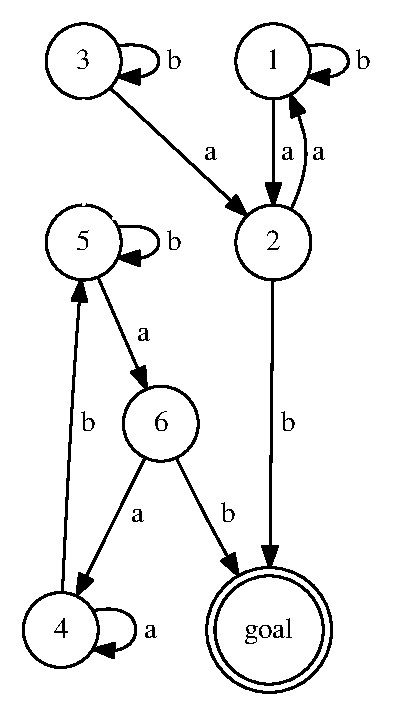
\includegraphics[width=0.6\columnwidth]{ExampleFSM} % Reduce the figure size so that it is slightly narrower than the column. Don't use precise values for figure width.This setup will avoid overfull boxes. 
%% \caption{An example Blind FSM}
%% \label{fig1}
%% \end{figure}


%% %  Here is the transition table for the FSM in the figure
%% %          a  b
%% %       1  2  1
%% %       2  1  G
%% %       3  2  3
%% %       4  4  5
%% %       5  6  5
%% %       6  4  G

%% The agent begins in a random, non-goal state.  It first takes action
%% 'b' and does not reach the goal as a result of this action.  While the
%% agent does not know the transition table of the FSM, we can look at
%% the diagram and know that the agent must have begun in state 1, 3, 4
%% or 5 and now must be in state 1, 3 or 5.  As a result, we know that
%% the agent is guaranteed to reach the goal in two steps if it takes the
%% action \textit{a} followed by \textit{b}.  This makes \textit{bab} a
%% universal sequence for this particular FSM.

%% \begin{comment}
%% \section{A Little Less State Aliasing}

%% % Do we need to discuss the lack of tuning parameters?

%% The situation changes once the agent is given additional sensors
%% beyond the goal sensor.  Consider an environment like Blind FSM but
%% the agent also has a binary sensor that tells it when it is currently
%% in an odd state or an even state.  We shall henceforth refer to this
%% as the OSFSM (Odd-Sensor Finite State Machine) environment.

%% For an OSFSM environment using the FSM in Figure \ref{fig1}, the
%% universal sequence (\textit{bab}) is sub-optimal.  The agent can
%% consistently reach the goal faster (or at least as fast) by always
%% taking action \textit{b} in even numbered states and action \textit{a}
%% in odd numbered states.  Thus, the MaRz algorithm needs to be enhanced
%% or replaced in such situations.

%% An episodic memory remains essential to be successful in the OSFSM
%% environment.  Traditional machine learning algorithms still perform
%% poorly in OSFSM since they can still only ever distinguish three
%% states.  However, as more and more sensors are provided a traditional
%% machine learning algorithm becomes more and more effective.  Thus,
%% there is a continuum from complete state aliasing (e.g., the Blind FSM
%% environment) to a fully observable environment.

%% The goal becomes to create an algorithm that can function well in
%% both.  This research presents ARO, an initial step toward such an
%% algorithm.

\section{ARO Overview}

We are now ready to present ARO, an algorithm designed for navigating
environments with extreme state aliasing such as Blind FSM and OSFSM.

%ARO can be described in three parts: a data structure to store
%episodic memories and to describe what is currently known about the
%position of the agent in the machine, a method to estimate the value
%of exploring vs exploiting based on the data gathered, and an
%algorithm to use the data structure and the explore-exploit heuristic
%to decide what action to perform.

\subsection{Rules}

ARO stores previous events in units called ``episodes." Each episode
consists of the tuple $(o, a)$, where $o$ is the observation $f(s)$
and $a$ is the action taken after the observation. In the OSFSM
environment, an example episode may be $(1,b)$. In this episode, the
agent was in an odd-numbered state and took action $b$. When the agent
reaches the goal, the action is irrelevant, so we denote such an
episode simply with ``G." In non-goal episodes, we concatenate the
tuple for brevity, so the above episode would be denoted ``1b".


Using these episodic memories, the agent records patterns of cause and
effect in a structure called a \textit{rule}. Rules are denoted like
this example: $$1a \rightarrow 1: 23\%.$$ This rule states that being
in an odd state and taking action $a$ ``caused" an odd state $23\%$ of
the time. The effect part of a rule is always in this same style, but
causes may be more complex. For example, consider this
rule: $$0b,1a \rightarrow 1: 6\%.$$

%This rules says that the agent taking action $a$ while being in an
%odd state that was reached by taking a $b$ from an even state has
%caused an odd state $6\%$ of the time. In general, a rule consists of
%a sequence of episodes as the ``cause", an observation $o \in O$ as
%an ``effect," and the probability that the cause produces the stated
%effect.

This rule states that being in an even state and performing action
$b$, then reaching an odd state and performing action $a$ has caused
the agent to reach an odd state $6\%$ of the time.


More formally, a rule consists of three parts: a sequence of episodes of any length known as the \emph{cause sequence}, an observation known as the \emph{effect}, and a probability. The cause sequence of a rule may be empty, which can be interpreted as the probability  that transitioning to a new state causes a particular observation. The number of episodes in the cause sequence of a rule is called the \textit{depth} of a rule.

The three examples for rules given in the background section may now be formally stated. We will use $*$ to denote any possible value.
\begin{itemize}
	\item $*a \rightarrow x: 100\%$
	\item $*a_0, xa_1 \rightarrow G: 100\%$
	\item $xa \rightarrow y: 50\%$ and $xa \rightarrow z: 50\%$
\end{itemize}

As we can see from the final example, it is often useful to consider
the set of all rules with the same cause sequence. This lets us
consider all possible outcomes from taking a particular action. We
call such a set of rules a \textit{rule group}.

We used a tree structure to store rules, but this choice does not
effect functionality in contrast to similar algorithms that use a
tree-based data structure \cite{McCallumUSM95,Shani2005}. So rather
than explain this tree, we merely define the function \scshape
GetRule \normalfont that takes as inputs both a cause sequence and an
effect then produces as an output the corresponding rule. We also
define the function \scshape GetRuleGroup \normalfont that takes a
cause sequence as an input and produces the corresponding rule group
as an output.

Since the agent does not have access to the underlying FSM, it cannot
compute the probabilities for rules exactly. This leaves us with two
choices for developing the rules: learned knowledge and expert
knowledge. For learned knowledge, the agent estimates the probability
using the rate at which the effect follows the cause sequence in
episodic memory. For example, if $0b$ occurs $10$ times in memory and
$0b,G$ occurs $3$ times in memory, then the agent would use the
rule $$0b \rightarrow G: 30\%.$$ Expert knowledge can be used instead
of this estimate if it is provided to the agent. \scshape
GetRule \normalfont does not distinguish between the source of the
rule when providing it to the agent.


%There are multiple rules with the same cause sequence. For instance, both $1a \rightarrow 0: 3$ and $1a \rightarrow G: 2$ may be rules. By comparing all rules with the same cause sequence, the agent can compute the probability that any particular effect will occur. We will call this set of rules a ``rule group." We define the function called \scshape GetRuleGroup\normalfont(episodes), which takes an array of episodes and returns the corresponding rule group.

%For a given sequence of episodes, many rule groups apply. For example, the sequence $1a,0a,1b$ has 4 rule groups apply: the group for the full sequence, the $0a,1b$ group, the $1b$ group, and the group for the empty sequence. Each will produce different probabilities of what will be observed next. The probabilities from the high-depth groups will be less accurate due to having less data, but can describe more sophisticated patterns than low-depth groups. The array of rule groups that currently apply is called ``current."

Now that we have a method for storing patterns of cause and effect, we can use this information to predict future outcomes and find the optimal move.

\subsection{Expected Value}

Given a sequence of previous episodes that have occurred and an observation, we can recursively compute the expected number of moves it will take to reach the goal. This is computed under the assumption that at each choice the agent may have in the future, it will make the best possible move. The algorithm is below.


\algrenewcommand\algorithmicindent{1.25em}
\begin{algorithmic}[1]
	\Function{EV}{Episode[] $episodes$, Observation $o$}
		\State $BestSum = \infty$
		\State $BestMove = \epsilon$
		\For{$a$ in $\alpha$}
			\State $Sum = 0$
			\State Let $next = (o, a)$ be a new episode.
			\State Let $nextSeq$ be $episodes$ appended by $next$
			\State $nextGroup =$ \Call{GetRuleGroup}{$nextSeq$} % Note: This looks awful because LaTeX spreads out spacing. This will need the full page to loook correct
			\If{$nextGroup$ is empty}
				\State $Sum = $ \Call{GetHeuristic}{~} \label{line:heuristic}
			\EndIf
			\For{$rule$ in $nextGroup$}
				\State Let $e$ be the effect of $rule$.
				\State Let $p$ be the probability of $rule$.
				\If{$e = G$}
					\State $Sum = Sum + p$
				\Else
					\State $Sum = Sum + p*($\Call{EV}{$nextSeq$, $e$} $ + 1)$
				\EndIf
			\EndFor
			\If{$Sum < BestSum$}
				\State $BestSum = Sum$
				\State $BestMove = a$
			\EndIf
		\EndFor
	\State \Return $BestSum$
	\EndFunction
\end{algorithmic}

This algorithm also computes the move that will take the fewest number of steps to reach the goal on average, stored in the $BestMove$ variable. Let \scshape GetBestMove \normalfont be a function that, when given the same inputs as \scshape EV\normalfont, will return the value of the $BestMove$ variable. The action returned by \scshape GetBestMove \normalfont will minimize the expected number of steps to the goal based on what the agent has learned about the environment, so we would expect this would minimize the average number of steps to the goal  over the long term. ARO uses this function to determine what action to make.
%The agent may call this function, supplying the most recent observation and an episode sequence ending at its most recent episode or an empty sequence. Thus, performing the action $BestMove$ can be used as a policy for the agent, and should minimize the average steps to goal based on what the agent has learned about the environment. In fact, this is exactly what ARO does. 

There are two aspects of this policy that are not yet
explained. First, we cannot compute an expected value for a move we
have never taken before. This case is dealt with in
line \ref{line:heuristic} of the code with the \scshape
GetHeuristic \normalfont function, which we will define below. Second,
there are multiple sequences the agent may pass into \scshape
GetBestMove\normalfont. For instance, if the most recent episodes are
$1a,0a$ and the last observation was $0$, the agent may call \scshape
GetBestMove\normalfont($[]$, $0$), \scshape
GetBestMove\normalfont($[0a]$, $0$), or \scshape
GetBestMove\normalfont($[1a, 0a]$, $0$). Each sequence may produce a
different recommendation, and the agent must choose which
recommendation to follow. These are the corresponding topics of the
next two sections.

\subsection{Explore Heuristic}
%Old version?
%Let us first deal with the case where we have no rules in a rule group and we must find the expected value. This occurs if the agent has never observed the sequence of episodes corresponding to the rule group. Let $e = (o, a)$ be the last episode in the rule group cause sequence and $seq$ be the rest of the sequence. This situation is equivalently described as follows: the agent has never recorded episodes in the sequence $seq$, then observed $o$ and performed action $a$. Thus, taking action $a$ can be considered an "exploration" by the agent. We therefore need to decide the value of exploring in this environment, which is clearly a bandit problem. Specifically, this is a contextual bandit problem with $seq$ and $o$ forming the context and the arms being the actions in $\alpha$. However, in this context

Let us first deal with the case where we must calculate an expected
value for a rule group containing no rules. This can be equivalently
stated as follows: ARO has never seen the episode sequence $episodes$
occur, then observed the observation $o$, and then performed some
action $a$. Furthermore, no expert has provided knowledge on what they
expect to occur in this scenario. Thus, taking action $a$ can be
thought of as an ``exploration" by the agent. The agent must choose
between exploring this new action and exploiting its existing
knowledge to reach the goal.

The explore-exploit tradeoff is well studied under the context of the
Multi-Armed Bandit problems \cite{Berry85} and has several known
solutions \cite{Sutton98,Kearns02,Brafman02}.  Research with regard to
explore-exploit in environments with extreme perceptual aliasing is
much more difficult.  A publication by a previous researcher in this
area stated ``Efficient exploration with hidden state is an extremely
difficult problem, and remains an area requiring
work.'' \cite{McCallumUSM95}

To compare the value of this exploration to other actions we have
taken, we must decide the value of exploring in the units of expected
value.  It is possible to find an estimate of the expected value by
using the rule group corresponding to removing the first episode from
$episodes$. However, repeating this process can lead to infinite depth
recursion. Rather than creating a suitable base case to make the
recursion finite, we instead attempt to estimate the value that this
recursion will return. Let $p$ denote the probability of reaching the
goal according to the $0$-deep rule $\rightarrow G : p$. We note that
if we were to continue recursion infinitely, the probability of
reaching the goal in any step should converge on $p$. If we estimate
that this probability holds constant on every step, then the number of
steps to goal follows a Geometric distribution with probability
$p$. This gives an expected value of $\frac{1}{p}$. To prevent
dividing by $0$, we add $1$ to the number of goals observed when
calculating $p$. Hence, we can now define the heuristic function:

\begin{algorithmic}[-1]
	
	\Function{GetHeuristic}{~}
		\State \Return $1/p$
	\EndFunction
	
\end{algorithmic}

As a benefit of this technique, we have derived a quantitative value
of exploration without using hyperparameters, in contrast to
traditional techniques cited above. This fact makes this technique
particularly suitable to online learning and artificial general
intelligence problems where hyperparameter tuning is not
desirable. Also of note is that $\frac{1}{p}$ nearly equals the
average number of steps to goal over the lifetime of the agent (they
are not equal because we must add one to the number of goals). This
means that ARO's explore-exploit solution has an intuitive
description: explore if the alternative is worse than average.

This intuitive idea appears in other contexts.  Notably, an algorithm
called POKER has been applied to the multi-armed bandit problem where
the agent is not able to test all the arms before a time horizon is
reached \cite{Vermore05}.  In this context, the value of an arm is
estimated based on the average value of other arms.



\subsection{Sequence Selection}

The agent may now calculate the best move given a sequence of recent
episodes. However, different sized sequences may produce different
results. If a large sequence is used, the episode sequence is more
likely to be rare in memory, producing unreliable
predictions. Furthermore, a long sequence may contain superfluous
information, which would imply that a more common and shorter sequence
would be a sufficient state identifier. With a small sequence, the
episode sequence may be too common for the agent to know where it is
in the machine or to determine if it is going in a loop, which could
cause undesirable behavior such as infinite looping. To resolve this
dilemma, ARO uses a greedy strategy of taking the episode sequence
that produces the smallest expected value. Hence, if the agent has
knowledge of a fast path to the goal, it will take it regardless of
sequence length. We expect this strategy to help reduce regret.

This alone, however, is not sufficient to prevent loops. At timestep
$t$, say the sequence $seq$ has the property \scshape
EV\normalfont($seq$) $ = x$, where $x$ is the minimal expected
value. Hence, the action \scshape GetBestMove\normalfont($seq$) is
performed. Let $nextSeq$ be $seq$ appended by the new episode
generated by performing that action. We found that the expected value
of $nextSeq$ in timestep $t+ 1$ can be higher than $x$, usually from
an improbable event informing the agent that it is farther from the
goal than the average case. When this occurred, we observed that the
agent would often switch to a shorter sequence with a better expected
value for a move recommendation. However, this is not because the
agent actually knows a faster path to goal, but because the agent
effectively ``forgets" that it is in a poor position. After the agent
has performed a few moves, it will again learn that it is in a poor
position and switch to a shorter sequence for a recommendation. By
repeating this behavior, the agent gets stuck in a loop.

To deal with this issue, we force the agent to deal with the bad event
by not letting the agent switch to a different sequence for a move
recommendation. In other words, if $seq$ was used to find the best
move at timestep $t$, then $nextSeq$ must be used to find the best
move at timestep $t+1$. There are two exceptions to this rule:
\begin{enumerate}
	\item The agent observes a goal. Because the agent is moved randomly upon reaching the goal state, there is no information to be gained by using a sequence with a goal observation.
	\item $nextSeq$ is unique. This implies the agent is in a novel scenario and the current sequence can provide no data to guide the agent.
\end{enumerate}

Using these procedures, we can now fully define the policy of ARO. We
define the global variable $prevSequence$, which stores the sequence
from the previous time step used to determine which action to take,
and is initialized to the empty sequence. ARO's policy is then
described in the following algorithm.

\begin{algorithmic}
	\Function{Policy}{Observation $o$}
		\If{$o = G$}
			\State Set $prevSequence$ to the empty sequence.
			\State \Return $\alpha$[0]
		\EndIf
		\State Let $e$ be the last episode.
		\State Let $seq$ be $prevSeq$ appended by $e$.
		\State Let $f$ be the frequency of $seq$ in episodic memory
		\If{$f = 1$ or $seq$ contains the episode $G$}
			\State Set $prevSeq$ to the sequence of recent episodes such that \Call{EV}{$prevSeq$, $o$} is minimized.
			\State \Return \Call{GetBestMove}{$prevSeq$}
		\Else
			\State $prevSeq = seq$
			\State \Return \Call{GetBestMove}{$prevSeq$}
		\EndIf
		
	\EndFunction
	
\end{algorithmic}

%Often, it is necessary for the agent to look ahead more than one action. For example, if a rule group indicates to the agent that there is a $35\%$ chance that making an $a$ will lead to an odd state, it may be helpful to see what the chances are for reaching the goal by making an $a$ or $b$ from such an odd state. To allow for such operations, rules are stored in a tree-like data structure defined as follows: a node of the tree consists of an observation, a frequency, and a mapping from $\alpha$ to an array of nodes, where no pair of nodes in an array use the same observation. The root of this tree is an array of tree nodes.


\section{Results}

To assess ARO, we compared its performance in the OSFSM environment to
that of two other algorithms: MaRz \cite{Rodriguez17} and Nearest
Sequence Memory \cite{McCallumNSM95}. Since these agents cannot incorporate knowledge engineering no rules were provided for ARO \textit{a priori}. Since we would expect that being provided expert rules would improve performance, this data can be seen as a worst-case outcome for ARO.

There were a few modifications to the implementation of ARO from the specification to improve memory usage and run time. First, we discovered that there was no need to record a rule if a prefix of the cause sequence was unique. If the prefix occurs again, we may look back through memory to create the rule on the fly. This modification does not effect the behavior of ARO. Second, we cache the result of \scshape GetEV \normalfont and \scshape GetBestMove\normalfont after every goal, which dramatically improves computation time. This technically deviates from the specification because the value of \scshape GetHeuristic \normalfont is saved and not recomputed. Since $1/p$ trends downward as the agent learns more, this means that the agent undervalues explores compared to the specification. We found the overall effect on the agent to be small.

Figure \ref{fig4} below shows the performance of all three agents in
the Blind FSM environment.  Figure \ref{fig5} shows the results for the OSFSM environment.  These results are shown for a FSM with
50 states and a three-letter alphabet (three possible actions per
state).  The ordinal measures successive trips to the goal.  The
abscissa measures the number of actions required to reach the goal on
that trip.

\begin{figure}[t]
  \centering
  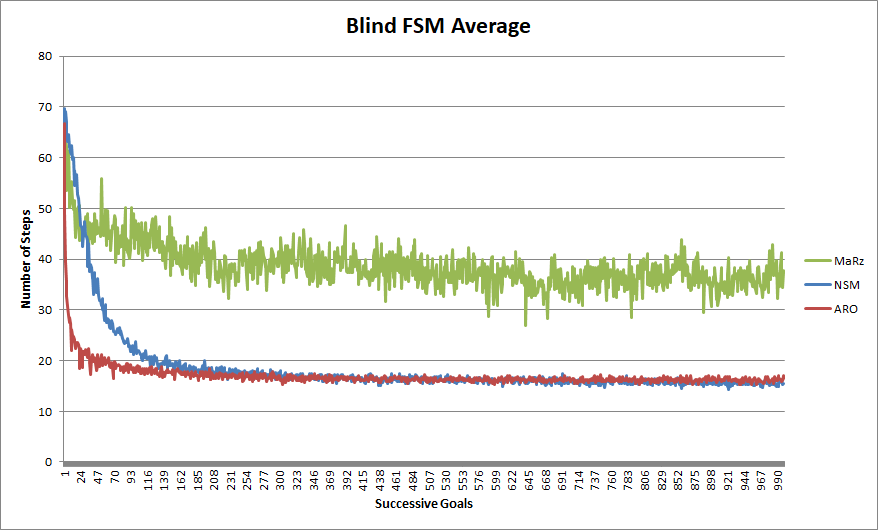
\includegraphics[width=0.9\columnwidth]{BlindFSMGraph.png} % Reduce the figure size so that it is slightly narrower than the column. Don't use precise values for figure width.This setup will avoid overfull boxes. 
  \caption{Agents in the Blind FSM Environment with 50 states and an alphabet size of 3. Data averaged from 1000 trials with random FSMs.}
  \label{fig4}
\end{figure}

\begin{figure}[t]
	\centering
	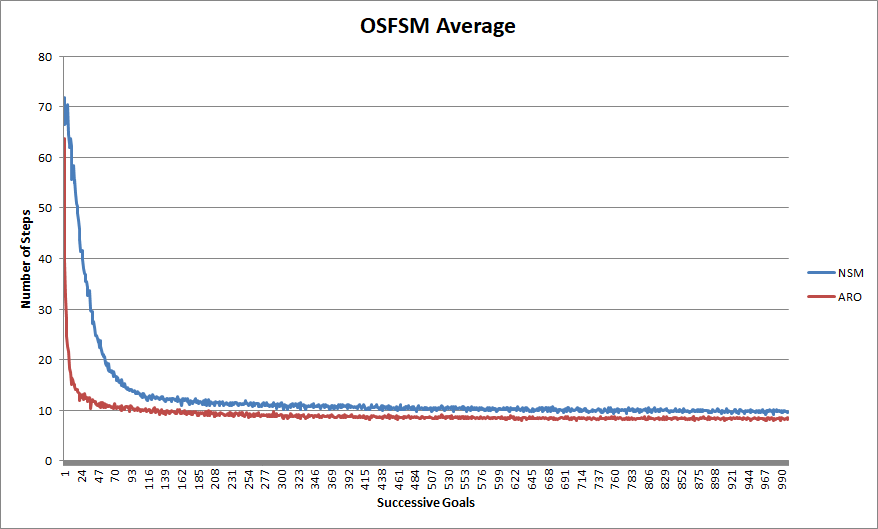
\includegraphics[width=0.9\columnwidth]{OSFSMGraph.png} % Reduce the figure size so that it is slightly narrower than the column. Don't use precise values for figure width.This setup will avoid overfull boxes. 
	\caption{Agents in the Odd-Sensor FSM Environment with 50 states and an alphabet size of 3. Data averaged from 1000 trials with random FSMs.}
	\label{fig5}
\end{figure}

Predictably, the number of steps to reach the goal declines
exponential on successive trips the goal indicating that the agent is
learning to improve its behavior.  This is true for all three
algorithms. MaRz learns faster than NSM for the first few goals but converges at a much less efficient policy.
ARO learns significantly faster than NSM and converges at a policy with nearly identical performance to NSM.

As shown, ARO is able to learn near optimal behavior much more rapidly
than the other algorithms.  These results were consistent across a
variety of different machines ranging from 10 to 90 states and
alphabets of 2 to 9 letters. (Note: some data for NSM was still being
gathered at the time of paper submission.)

\section{Future Work}

This work demonstrates that ARO is effective in two specific
environments with extreme state aliasing. Other tests (not in this
paper) have indicated that ARO can handle other deterministic
environments as well, including environments with little state
aliasing.

The most pressing concern is that it is not obvious how best to
generalize ARO to accommodate a stochastic observation function, such
as a function that returns $0$ or $1$ at random. With a random
observation function, storing all possible rules can quickly become
infeasible in terms of memory because the number of rules with a given
depth is exponential and unbounded. This is unlike a deterministic
observation function, where the number of rules with a given depth is
no greater than the total number of states of the FSM - one rule
corresponding to each possible initial state of the agent at the
beginning of the cause sequence. Furthermore, ARO has no means of
recognizing that the observations it receives are random, so it uses
rules trying to predict the value of random observations as a basis to
try to reach the goal. These factors cause ARO to perform poorly.

Another potential enhancement is to allow ARO to learn other kinds of
rules with more general causes or effects. For example, in our
previous examples of rules we used a wildcard character for a
rule. While this rule can be provided by an expert, ARO cannot learn
such a rule and must instead learn a similar rule for every possible
value of the wildcard.

ARO may also need to be adjusted to address environment with these
properties:
\begin{itemize}
\item a reward function rather than a single goal state
\item a non-deterministic FSM
\item a dynamic transition table
\item continuously valued sensors
\end{itemize}

ARO's applicability extends beyond knowledge integration.  As an
online algorithm, ARO can take advantage of knowledge immediately and
therefore could be step towards ways in which humans and artificially
intelligent agents work collaboratively on a given task in real time.

In addition, the development of ARO builds upon previous research to
explore the application of episodic memory for artificial general
intelligence \cite{Rodriguez17}.  ARO, therefore, is likely equally
applicable in that context.  In particular, the lack of
hyperparameters means that it can be applied in a general context and
does not need to be re-tuned each time it is used in a new
environment.



\begin{quote}
\begin{small}
\bibliographystyle{aaai}
\bibliography{aro}
\end{small}
\end{quote}

\end{document}
